% #############################################################################
% This is Chapter 2
% !TEX root = main.tex
% #############################################################################
% Change the Name of the Chapter i the following line
\fancychapter{Background}
\clearpage
% The following line allows to ref this chapter
\label{chap:chap002}

This chapter (Chapter~\ref{chap:chap002}) contains useful information about the background of the breast cancer domain considered in the context of this thesis.
However, it does not describe any original contributions and can be skipped if the reader is acquainted with the background.

\section{Medical Imaging Diagnosis}
\label{sec:chap002001}

Screening aims to identify cancer at earlier stages of the several diseases, when treatment can be more successful~\cite{McKinney2020}.
However, two main difficulties arise.
First, the amount of data to be processed has been increasing significantly and greatly surpasses the throughput capabilities of the radiologists~\cite{HANNA20181709}.
Second, processing such amount of data in a timely fashion without compromising the reliability of the diagnosis is very challenging~\cite{waite2017systemic, stec2018systematic}.
These difficulties have been the driving force behind the recent trend in {\it radiomics}\footnotemark[4] (Section~\ref{sec:chap002006}) and the integration of \ac{AI} techniques into medical imaging~\cite{Lambin2017, pesapane2018artificial, doi:10.1148/radiol.2015151169}.

%%%%%%%%%%%%%%%%%%%%%%%%%%%%%%%%%%%%%%%%%%%%%%%%%%%
\footnotetext[4]{Involving the high-throughput extraction of quantitative imaging features, {\it radiomics} intent of creating mining information from radiological images. Large-scale data sharing is necessary for the validation and full potential that {\it radiomics} represents.}
%%%%%%%%%%%%%%%%%%%%%%%%%%%%%%%%%%%%%%%%%%%%%%%%%%%

\section{Breast Cancer Domain}
\label{sec:chap002002}

In the context of breast cancer, the requirements for multi-modal data have a significant impact on the clinical workflow~\cite{10.1117/1.JBO.22.4.046008}.
Although \ac{MG} is the primary imaging modality for breast screening, it may be insufficient to reach a correct diagnosis.
For instance, in dense breasts (Figure~\ref{fig:fig005} {\bf B}, {\bf D}), the lesions can hardly be seen~\cite{10.1093/jbi/wbaa010}, while in adipose breasts, lesion visualization is clear (Figure~\ref{fig:fig005} {\bf A}, {\bf C}).
Thus, for dense breasts, other modalities constitute a valuable information to complement the diagnosis.
Figure~\ref{fig:fig005} {\bf E}, {\bf F} depicts the \ac{US} and \ac{DCE}-\ac{MRI} modalities, where the lesions can be easily viewed.
Among all these imaging characteristics, classifying a tumor into benign or worrisome categories (severity) is the ultimate objective~\cite{SHAN2016980}.
Next (Section~\ref{sec:chap002003}), this document explains how the severity classification works for the breast cancer diagnosis.

%%%%%%%%%%%%%%%%%%%%%%%%%%%%%%%%%%%%%%%%%%%%%%%%%%
\begin{figure}[htbp]
\centering
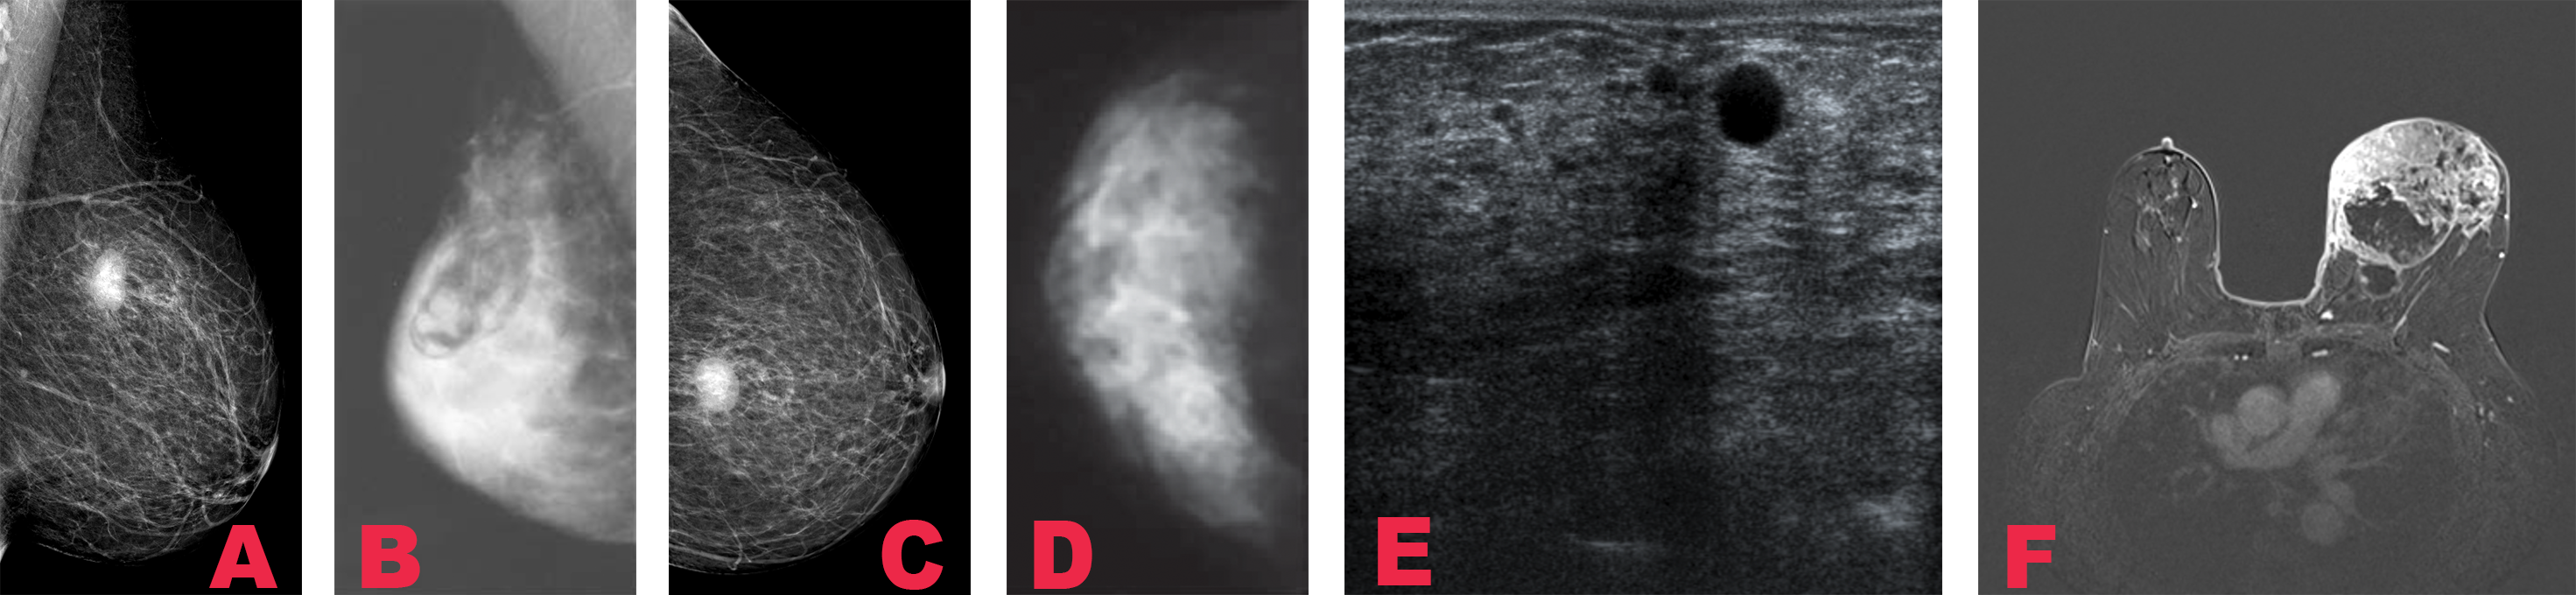
\includegraphics[width=\columnwidth]{images/fig005}
\caption{Illustration of the current clinical setup. Adipose breast in MG where the lesions are easily viewed (A, C). Dense breast where is not possible to view the lesions (B, D). In the latter scenario, the radiologists resort to other image modalities such as US (E) and DCE-MRI (F), to complement the information that is missing in (B, D).}
\label{fig:fig005}
\end{figure}
%%%%%%%%%%%%%%%%%%%%%%%%%%%%%%%%%%%%%%%%%%%%%%%%%%

\section{Severity Classification}
\label{sec:chap002003}

Clinical guidelines recommend regular image screenings to assess the risk of breast cancer~\cite{MIAO201817}.
To reduce variations in the radiologists’ descriptions of imaging findings, the \href{https://www.acr.org/}{\ac{ACR}} developed the \ac{BI-RADS}~\cite{d2018breast}.
The \ac{BI-RADS} provides a standard lexicon (Figure~\ref{fig:fig020}) to describe imaging findings and a classification system with six categories\footnotemark[5] to assess the likelihood of malignancy.

%%%%%%%%%%%%%%%%%%%%%%%%%%%%%%%%%%%%%%%%%%%%%%%%%%%
\footnotetext[5]{\ac{BI-RADS}: stands for \acf{BI-RADS}, which is a scale for putting the findings from breast cancer diagnosis into a small number of well-defined categories. The scale ranges from 0 to 6 (see more at \hyperlink{https://breast-cancer.ca/bi-rads/}{breast-cancer.ca/bi-rads}). However, for the simplicity of the study, we just considered a 1 to 5 scale range. Radiologists can only score a 6 after biopsy and the 0 means that the study need additional imaging.}
%%%%%%%%%%%%%%%%%%%%%%%%%%%%%%%%%%%%%%%%%%%%%%%%%%%

%%%%%%%%%%%%%%%%%%%%%%%%%%%%%%%%%%%%%%%%%%%%%%%%%%
\begin{figure}[htbp]
\centering
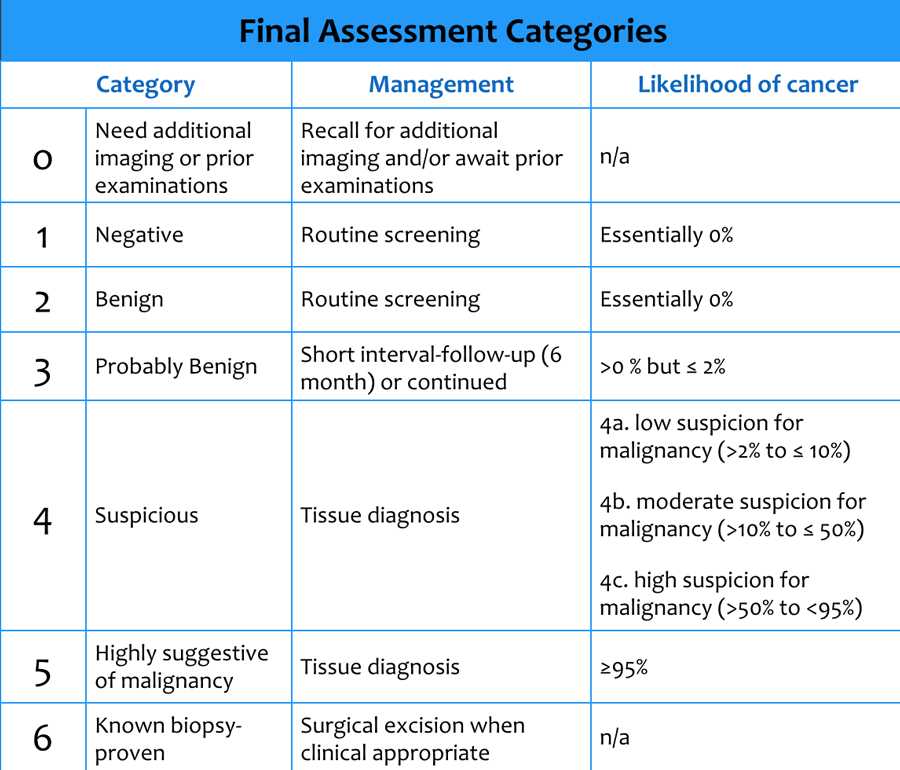
\includegraphics[width=\columnwidth]{images/fig020}
\caption{The BI-RADS enables radiologists to communicate results clearly and consistently, with a final assessment and specific recommendations. Image from \protect\href{https://radiologyassistant.nl/breast/bi-rads/bi-rads-for-mammography-and-ultrasound-2013}{radiologyassistant.nl} in November 2020.}
\label{fig:fig020}
\end{figure}
%%%%%%%%%%%%%%%%%%%%%%%%%%%%%%%%%%%%%%%%%%%%%%%%%%

In this thesis, a \ac{DNN} was trained to assess \ac{BI-RADS} breast classification.
Chapter~\ref{chap:chap006} will detail the number of screening patients and images, as well as its importance of assessing these categories.

\section{Lesion Typification}
\label{sec:chap002004}

The lesion typification~\cite{doi:10.1148/radiol.2018181371} is also a challenge to address in this thesis background.
The goal of this section is to explain what is the importance of the lesions, {\it i.e.}, masses (Section~\ref{sec:chap002004001}) and the microcalcifications (Section~\ref{sec:chap002004002}), that will feed the \ac{AI} algorithms (Chapter~\ref{chap:chap005} and Chapter~\ref{chap:chap006}) and provide visual information to clinicians.
For the severity classification~\cite{8611096, 9231684}, it is important to know the type of mass shapes, microcalcification patterns, and size to understand its importance to the algorithms.

\subsection{Masses}
\label{sec:chap002004001}

Concerning the mass typification (Figure~\ref{fig:fig021}), the benign masses are either round, oval, or lobular shapes, and the malign masses are either lobular, irregular, or architectural distortion shapes~\cite{nadia2020xai}.
The margins can also tell us information about the lesion.

%%%%%%%%%%%%%%%%%%%%%%%%%%%%%%%%%%%%%%%%%%%%%%%%%%
\begin{figure}[htbp]
\centering
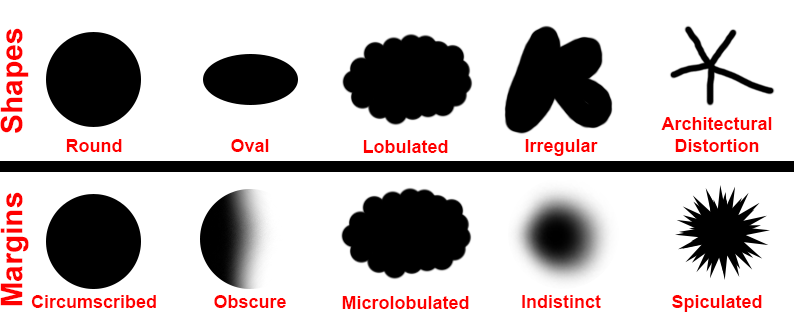
\includegraphics[width=\columnwidth]{images/fig021}
\caption{[DOI: \href{https://doi.org/10.13140/RG.2.2.33693.26086}{10.13140/RG.2.2.33693.26086}] Lesion Types~\cite{nadia2020maivelt} - First line is showing the type of {\bf Shapes}: {\bf Round}, {\bf Oval}, {\bf Lobulated}, {\bf Irregular}, and {\bf Architectural Distortion}. The second line is showing the type of {\bf Margins} of the lesion: {\bf Circumcribed}, {\bf Obscure}, {\bf Microlobulated}, {\bf Indistinct}, and {\bf Spiculated}.}
\label{fig:fig021}
\end{figure}
%%%%%%%%%%%%%%%%%%%%%%%%%%%%%%%%%%%%%%%%%%%%%%%%%%

There are five types of margins.
The circumscribed represents a benign margin.
The microlobulated, indistinct, and spiculated are suspicious findings, where the last one represents the most suspicious.
Finally, we have the obscured margin.
In this case, part of the margin is hidden by fibroglandular tissue.
If a patient case has an obscured margin result, the suggested action (Figure~\ref{fig:fig018}) is to perform an \ac{US}.

\subsection{Microcalcifications}
\label{sec:chap002004002}

Regarding the typification of the microcalcifications, there are five types~\cite{nadia2020xai}.
In this section, the document will explain the patterns (Figure~\ref{fig:fig022}) from the less malign to the most malign.

First of all, the diffuse pattern (letter {\bf a} of Figure~\ref{fig:fig022}) means that microcalcifications are dispersed randomly throughout the breast.
Second, the regional pattern (letter {\bf b} of Figure~\ref{fig:fig022}), when several microcalcifications are occupying over two centimeters of the breast.
Next, the group pattern (letter {\bf c} of Figure~\ref{fig:fig022}) is a small amount of microcalcifications in a small area of the breast.
The linear pattern (letter {\bf c} of Figure~\ref{fig:fig022}), that forms a line, may mean that the microcalcifications are deposited in a duct.
Lastly the segmental pattern (letter {\bf d} of Figure~\ref{fig:fig022}), meaning that the microcalcifications are deposited in the duct or several ducts, and their branches respectively.

%%%%%%%%%%%%%%%%%%%%%%%%%%%%%%%%%%%%%%%%%%%%%%%%%%
\begin{figure}[htbp]
\centering
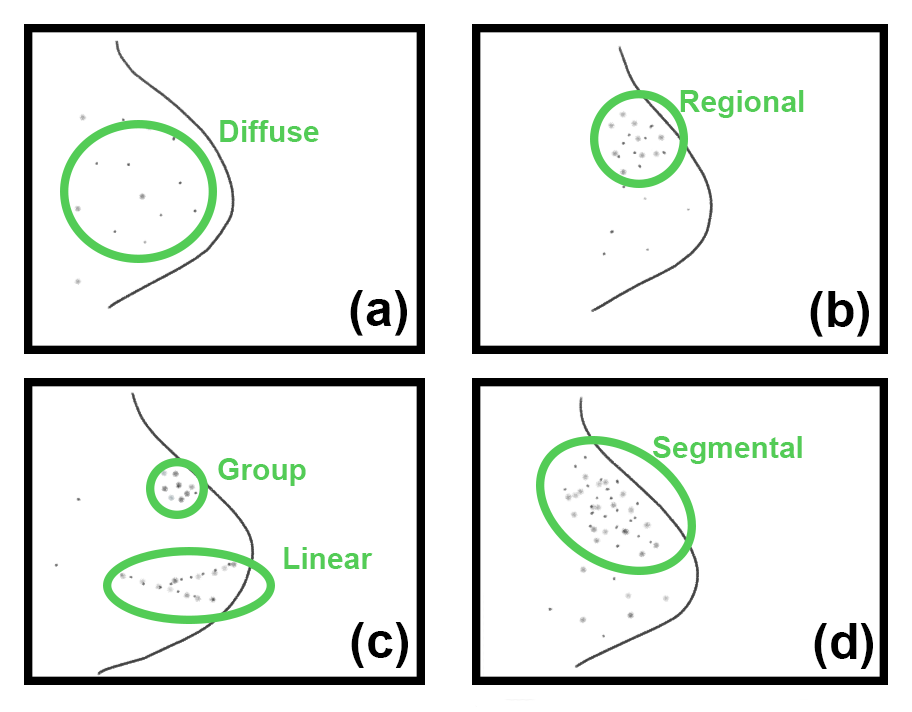
\includegraphics[width=\columnwidth]{images/fig022}
\caption{[DOI: \href{https://doi.org/10.13140/RG.2.2.26667.80164}{10.13140/RG.2.2.26667.80164}] Calcification Types~\cite{nadia2020maivect} - The {\bf Diffuse} is when the microcalcifications are ``randomly'' spreaded across the image. The {\bf Regional} is when the microcalcifications are close to each other forming a sort of a ``circle''. The {\bf Group} is a small area with few microcalcifications. The {\bf Linear} is when the microcalcifications form ``lines''. The {\bf Segmental} is similar to the {\bf Regional} but approaching a more oval shape instead of a circular.}
\label{fig:fig022}
\end{figure}
%%%%%%%%%%%%%%%%%%%%%%%%%%%%%%%%%%%%%%%%%%%%%%%%%%

In the context of breast cancer, the requirements for multimodality have a significant impact on the clinical workflow~\cite{https://doi.org/10.1002/cncr.32910}.
Although \ac{MG} is the primary imaging modality (Figure~\ref{fig:fig018}), it may be insufficient to reach a correct and complete dataset for clinicians and for \ac{AI}~\cite{DANA2020541}.
Next (Section~\ref{sec:chap002005}), the document explains the current imaging workflow and the importance of having a multi-modal available data.

\section{Radiology Reading Room}
\label{sec:chap002005}

The main \ac{RRR} workflow (Figure~\ref{fig:fig018}) can be defined as a three-stage process:
(1) {\it examination};
(2) {\it diagnosis}; and
(3) {\it report}.
The {\it examination} stage (Section~\ref{sec:chap002005001}) refers to the time spent on the examination and processing of the patient records ({\it e.g.}, demographics, clinical records or past medical images).
For instance, the radiologist receives this information from both the hospital and radiology information systems~\cite{islam2018recent}.
The second stage, {\it i.e.}, {\it diagnosis} (Section~\ref{sec:chap002005002}), corresponds to the time that the radiologist spends on the interpretation and diagnosis of the patient exams.
In this phase, the radiologist interacts with a \ac{PACS} retrieving the {\it modality working list} from a radiology information system~\cite{DIROBERTO2016950} of the hospital.
Finally, in the last stage, {\it i.e.}, {\it report} (Section~\ref{sec:chap002005003}), it refers to the time spent on reporting her/his conclusions after the patient's medical images analysis.

%%%%%%%%%%%%%%%%%%%%%%%%%%%%%%%%%%%%%%%%%%%%%%%%%%%
\begin{figure}[htbp]
\centering
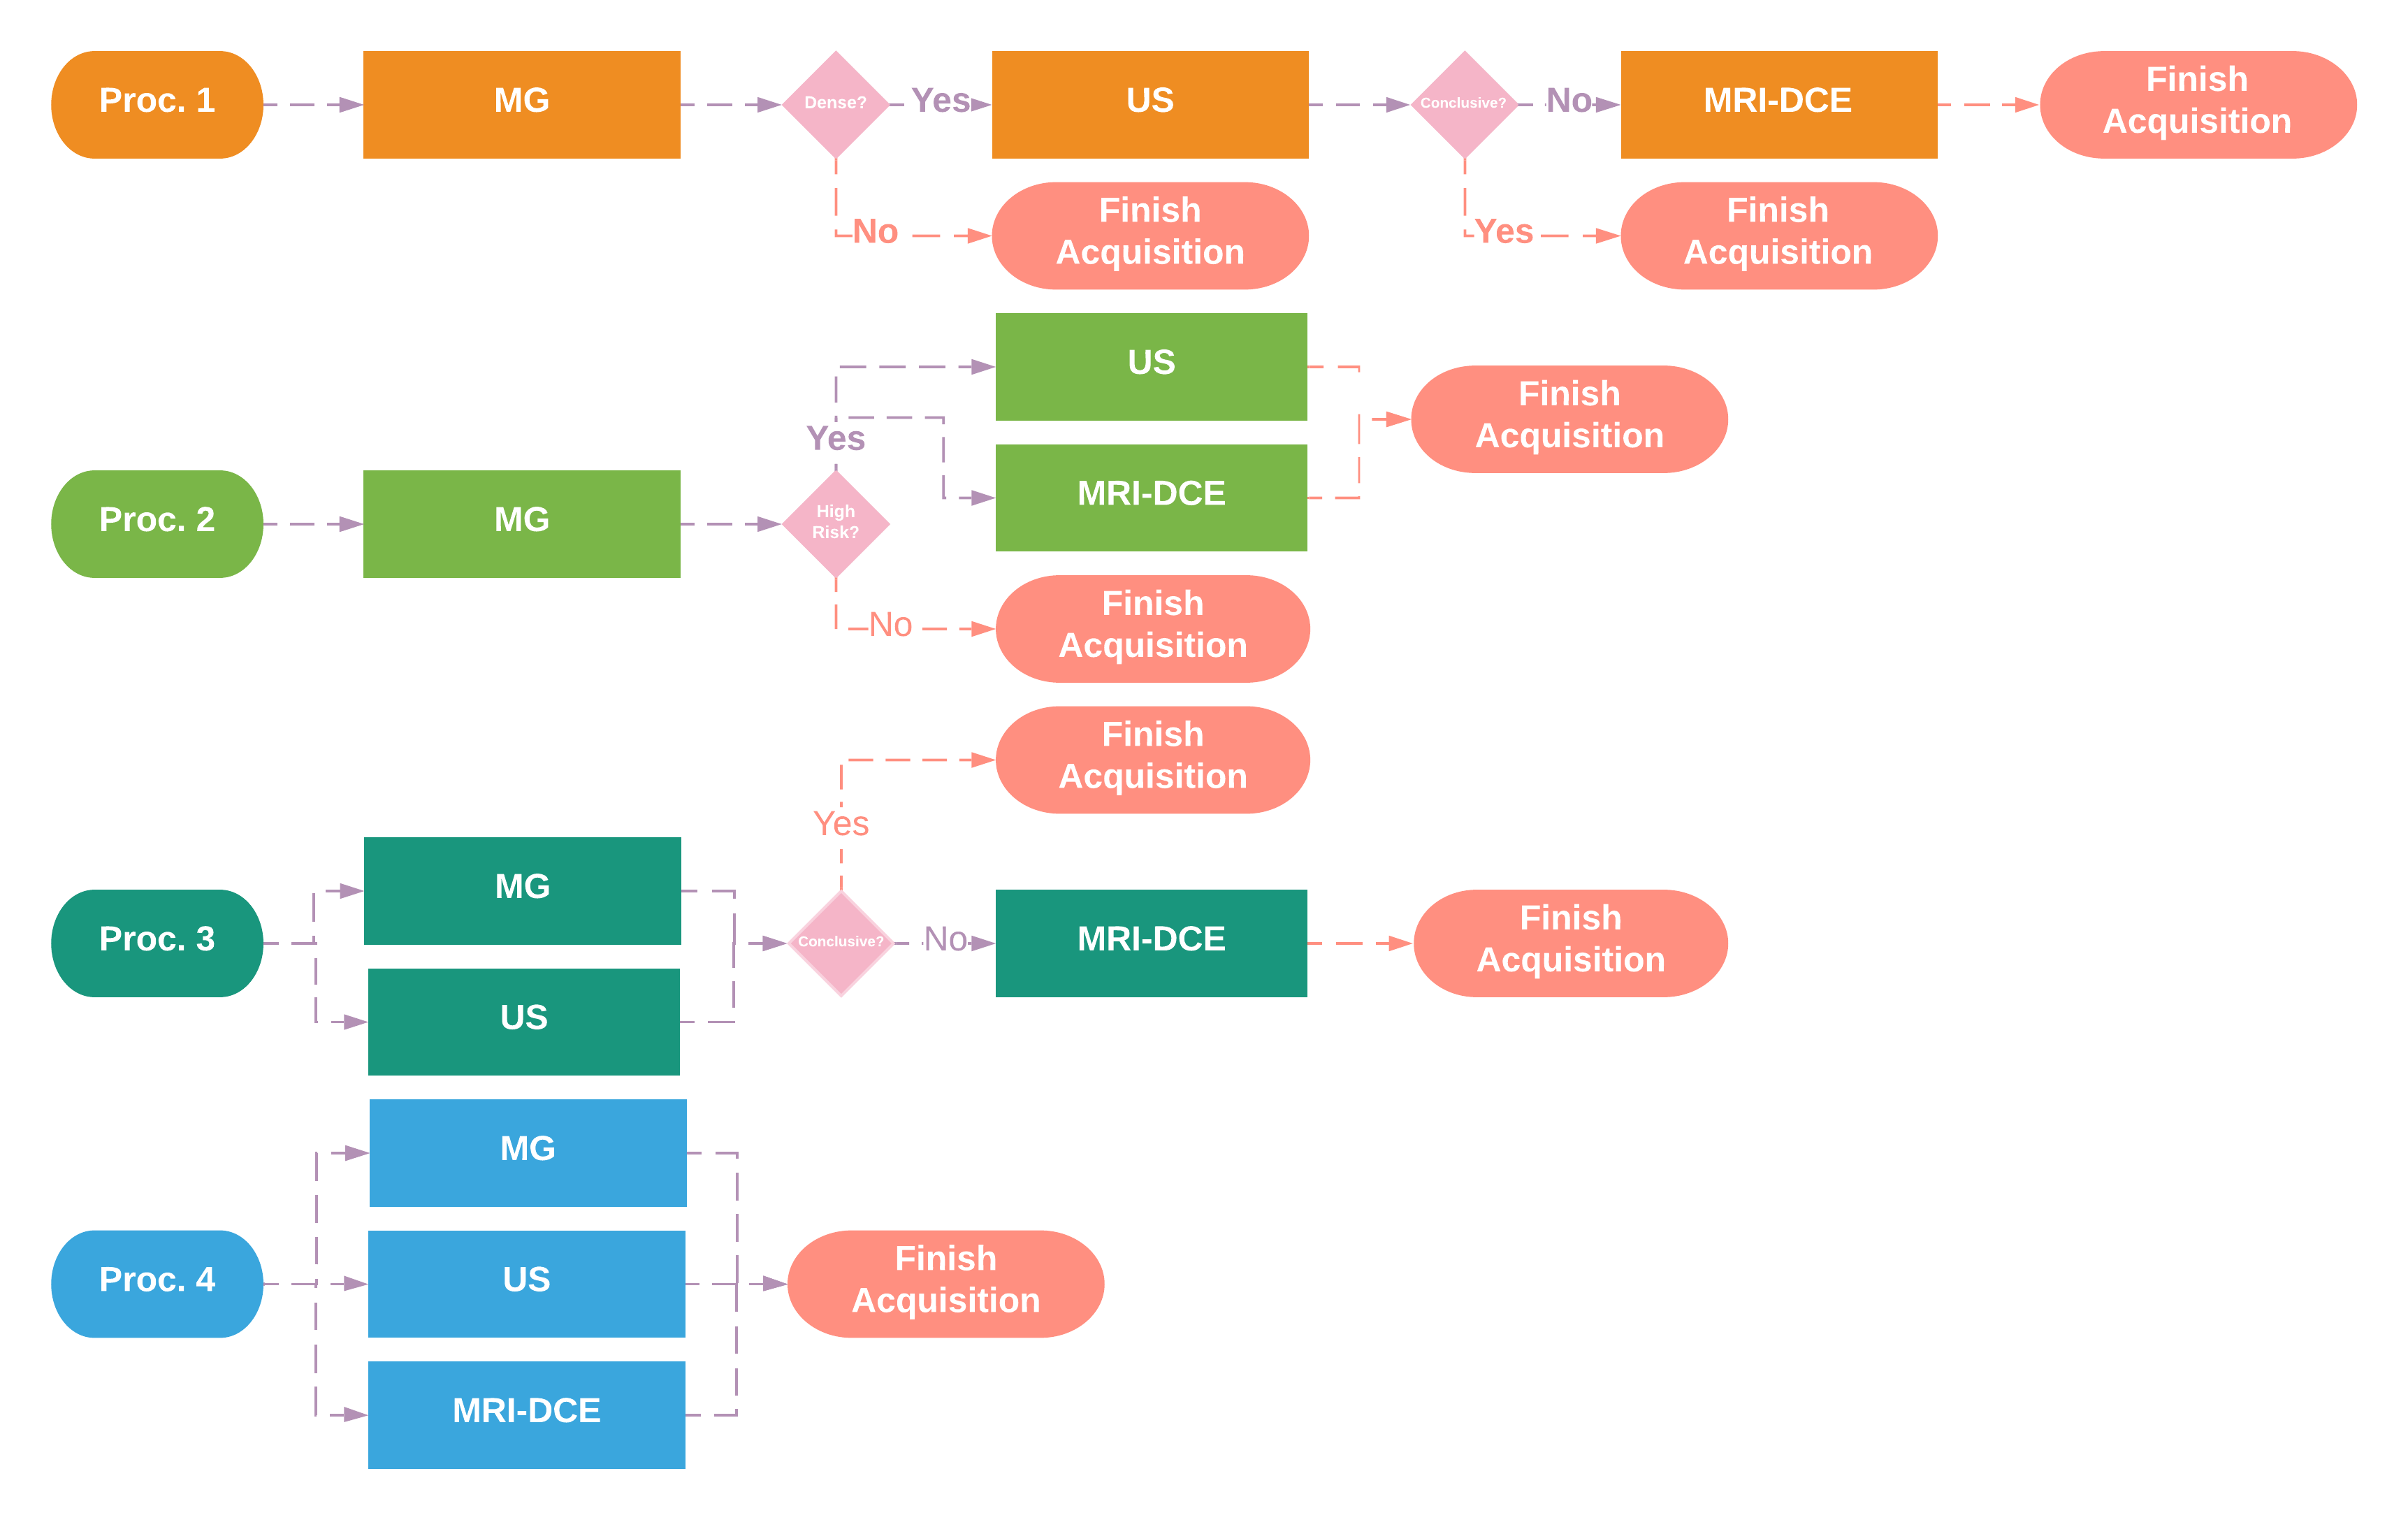
\includegraphics[width=\columnwidth]{images/fig018}
\caption{Workflow of the radiology reading room is commonly adopted in current clinical institutions using several image acquisition strategies. Screening modalities ({\it e.g.}, US, MRI, etc) constitute important complementary information for a reliable diagnosis.}
\label{fig:fig018}
\end{figure}
%%%%%%%%%%%%%%%%%%%%%%%%%%%%%%%%%%%%%%%%%%%%%%%%%%%

In all the above stages, images are used with different purposes, as described next.
The stages will be important to identify and define each workflow of the nine clinical institutions (Chapter~\ref{chap:chap005}) that collaborated in these studies.
Next, we describe each stage in detail.

\subsection{Image Examination}
\label{sec:chap002005001}

For the {\it examination} stage~\cite{8621479}, the clinician relates medical imaging analysis with other exams and medical records, {\it i.e.}, the clinical situation of the patient.
The {\it examination} of the patient is sometimes supported by other systems that give the clinician a more reliable source of information~\cite{islam2018recent, DIROBERTO2016950}.
Most of the information sought is stored in various formats~\cite{GIBSON2018113}, including notes from the referring physician (the doctor who sent the patient to the radiology department), past exams and respective reports, and second opinion from other clinicians.

\subsection{Patient Diagnosis}
\label{sec:chap002005002}

Regarding the {\it diagnosis} stage~\cite{https://doi.org/10.1002/cncr.32872}, this is the most crucial from this document perspective, since it is the one that most contributes to the treatment choice.
The {\it diagnosis} stage includes image classification (Section~\ref{sec:chap002003}) by using the \ac{BI-RADS} scale.
During this stage, clinicians were observed on the diagnosis process, namely accessing several medical images.
Several studies were conducted (Chapter~\ref{chap:chap005}) to understand what clinicians need during decision-making and while interacting with an intelligent agent.
At this stage, every 2D medical imaging modality takes about 120 seconds to be analysed, meaning that the clinician takes about two minutes to interpret each imaging type~\cite{jiang2018interpretation}.
However, in most of the cases, each patient requires more than six 2D images and several other 3D volume sequences\footnotemark[6] to be analysed ({\it e.g.}, the MRI volumes can have more than 100 frames per each sequence).
This means that a complete diagnosis in a real situation ({\it i.e.}, reading all modalities, clinical records and reporting the patient case) can take more than an hour of the clinician's time~\cite{Forsberg2017}, making this task cumbersome in the overall time of the {\it diagnosis} and prone to errors.
In observations, it was concluded that most of the clinicians disengage from visualizing all set of medical images, or disregard some pathologies in the images.
These handicaps may cause human errors and medical distractions~\cite{bruno2015understanding}.

%%%%%%%%%%%%%%%%%%%%%%%%%%%%%%%%%%%%%%%%%%%%%%%%%%%
\footnotetext[6]{The \ac{MRI} volumes comprises different types of sequences, concretely, T1, T2, T2 Fat Sat, Diffusion, \ac{DCE}-\ac{MRI}, \ac{DCE}-\ac{MRI} with subtraction in five time instants. The sensitivity of \ac{MRI} makes it an excellent tool in specific clinical situations. Situations such as the screening of patients at high risk, and evaluation of the extent of disease in patients with a new diagnosis. Compared to \ac{MG} and \ac{US}, \ac{MRI} provides higher sensitivity, however its specificity is variable. Moreover, \ac{MRI} data analysis is time-consuming and depends on reader expertise.}
%%%%%%%%%%%%%%%%%%%%%%%%%%%%%%%%%%%%%%%%%%%%%%%%%%%

\subsection{Final Report}
\label{sec:chap002005003}

After a patient classification, the clinician takes into consideration the first and the second stages ({\it i.e.}, {\it examination} and {\it diagnosis}) to improve the patient's clinical records and determine the prognosis~\cite{segrelles2017increasing}.
During the classification phase, the clinician examines the patient records and, by analyzing each medical image, records the {\it report} in a dictating system~\cite{SENG202079}.
The records are transcribed to a report, which are reviewed later by clinicians (signing the report as final).
After a patient classification, the clinician takes into consideration the first and the second stages ({\it i.e.}, {\it examination} and {\it diagnosis}) to improve the patient's clinical records and determine the prognosis.
The records are transcribed to a {\it report}, which are reviewed later by clinicians (signing the report as final).

\subsection{Summarizing Clinical Procedures}
\label{sec:chap002005004}

As previously discussed, using images to display breast lesions vary widely across medical imaging modalities (\ac{MG}, \ac{US} and \ac{DCE}-\ac{MRI}, being the two latter modalities crucial for dense breasts).
Multimodality is responsible for increasing the cognitive load of radiologists and increasing detection rates, but also reducing \acp{FP} and \acp{FN}~\cite{cheung2017integral}.
In this section, we define and describe the main clinical procedures.

\hfill

\noindent
The main clinical procedures (Figure~\ref{fig:fig018}) of the \ac{RRR}~\cite{wagner2015analysis} workflow usually comprises four different paths that correspond to different observed image acquisition procedures:

%%%%%%%%%%%%%%%%%%%%%%%%%%%%%%%%%%%%%%%%%%%%%%%%%%%
\begin{enumerate}
\item \textbf{Procedure 1} starts with the acquisition of \ac{MG}, then, if the breast is dense, the \ac{US} modality is acquired. Finally, if the \ac{MG} and \ac{US} are not conclusive, the \ac{DCE}-\ac{MRI} is acquired, otherwise the process is concluded;
\item \textbf{Procedure 2} starts with the acquisition of \ac{MG}, then if the clinician detects a high risk of cancer from the image patterns and/or patient records, both \ac{US} and \ac{DCE}-\ac{MRI} are acquired, otherwise the process is concluded;
\item \textbf{Procedure 3} \ac{MG} and \ac{US} are acquired simultaneously, if the {\it exam} is still not conclusive, the \ac{DCE}-\ac{MRI} is acquired;
\item \textbf{Procedure 4} all three modalities (\ac{MG}, \ac{US} and \ac{DCE}-\ac{MRI}) are acquired simultaneously.
\end{enumerate}
%%%%%%%%%%%%%%%%%%%%%%%%%%%%%%%%%%%%%%%%%%%%%%%%%%%

\hfill

From the interviews and observations (Chapter~\ref{chap:chap005}), it was found that radiologists access medical images in two main scenarios:
i) imaging perception process, namely to detect patterns of lesions;
and ii) finding relationships between past lesion patterns and possible future diagnosis.
Given the time constraints and the amount of information available, clinicians often do not observe all the images with the necessary detail.
From these observations (Chapter~\ref{chap:chap005}), it was concluded that they start by analyzing the patient's clinical history (when available).
In the end, the clinical history provides the necessary knowledge on how to guide the analysis of the current state and the basis of {\it radiomics}.
In the next section, the document will introduce the basics and definitions of the {\it radiomics} topic.

\section{Radiomics}
\label{sec:chap002006}

The topic of {\it radiomics} is a growing field that aims at extracting and mining the information from medical images~\cite{van2020radiomics}.
Specifically, the goal is to develop computerized support systems to improve the clinical decision-making.
Among the clinical tasks, breast cancer diagnosis is one of the main areas where {\it radiomics} is most growing~\cite{valdora2018rapid}.

\ac{CADx} systems can be developed to improve the diagnostic pipeline through automatic tumor malignancy assessment and reduction of negative diagnostic rates.
Through these \ac{CADx} systems, the application of {\it radiomics} to breast cancer may result in the acquisition of important information for feature modelling~\cite{10.1007/978-3-030-59716-0_71}.
The introduction of intelligent agents for feature modelling in \ac{CADx} systems will result in a better breast cancer characterization.
An accurate communication of intelligent agents will have the potential to improve diagnostic performance by a decrease in sensitivity and specificity of the medical errors~\cite{doi:10.1148/radiol.2020192039}.
For breast tumor classification (Section~\ref{sec:chap002003} and Section~\ref{sec:chap002004}), this section needs to also address the {\it radiomics} pipeline (Figure~\ref{fig:fig023}) that will be employed to extract imaging features from tumor images.

%%%%%%%%%%%%%%%%%%%%%%%%%%%%%%%%%%%%%%%%%%%%%%%%%%%
\begin{figure}[htbp]
\centering
\includegraphics[width=\columnwidth]{images/fig023}
\caption{Breast tumors are analyzed through this pipeline, where {\it radiomics}, paired with AI, ML and DL techniques is of chief importance, to recognize image-based patterns and perform the diagnostic classification based on quantitative imaging features.}
\label{fig:fig023}
\end{figure}
%%%%%%%%%%%%%%%%%%%%%%%%%%%%%%%%%%%%%%%%%%%%%%%%%%%

Several techniques are employed to analyse (letter {\bf a} of Figure~\ref{fig:fig023}) imaging features.
From tumor images, automatic segmentation can delineate the lesion contours (Figure~\ref{fig:fig021}), as well as extract texture, shape, and margin (Section~\ref{sec:chap002004001}).
With these feature extraction (letter {\bf c} of Figure~\ref{fig:fig023}), the descriptors of {\it radiomics} can characterize, {\it i.e.}, detect (letter {\bf b} of Figure~\ref{fig:fig023}) and classify (letter {\bf d} of Figure~\ref{fig:fig023}), the lesion.
Further, it will be possible to compare the autonomous with the clinician characterization.

In this thesis, several {\it radiomics} are extracting quantitative features to train a variety of classifiers.
The aim is to extract the quantified characteristics for an available and curated dataset (Chapter~\ref{chap:chap004}) of breast images with the aid of automated algorithms and respective intelligent agents.
There has been numerous pipelines and methods developed, although the lack of standardization in medical image processing makes it difficult to consume different formats.
Thus, in Section~\ref{sec:chap002007} this challenge is addressed.

Despite the success of \ac{DL}, and even though different studies have shown that {\it radiomics} ({\it i.e.}, \ac{AI}-assisted methods for medical image analysis) can reduce human error and improve outcomes~\cite{Cai:2019:HTC:3290605.3300234, delvaux2017effects, middleton2016clinical}, their adoption by the medical community has been slow.
One of the main reasons is the inability of these systems to provide relevant medical information or to capture the nuances of the human mind~\cite{khairat2018reasons, kohli2018cad, 10.1145/2858036.2858373}, making them untrustworthy and preventing their clinical acceptance.
In particular, \ac{DL}-based methods have been frequently viewed as `black box' approaches~\cite{litjens2017survey}.
Therefore, \ac{HCI} play an important role in creating user-friendly interactive systems for \ac{AI}-assisted medical image analysis~\cite{10.1145/3132272.3134111}.

\section{Medical Imaging Standards}
\label{sec:chap002007}

The \ac{DICOM} format\footnotemark[7] is normally used to store medical images~\cite{Trivedi2019} and is a standard in medicine.
Supporting a wide variety of medical information ({\it e.g.}, exam images, structured reports, etc), it also has the benefit to convert known file formats, such as \ac{JPEG} and \ac{MPEG}.
The medical information encoded by a \ac{DICOM} file (Figure~\ref{fig:fig025}) is called a dataset and takes the form of an associative array.
Each value can itself be a list of datasets (Chapter~\ref{chap:chap004}), leading to a hierarchical data structure that is much like a \ac{JSON} file.
In the \ac{DICOM} terminology, each key is called a \ac{DICOM} tag.
The list of the standard \ac{DICOM} tags is normalized by an official dictionary.
For improved readability, it is also common to name these \ac{DICOM} tags ({\it e.g.}, \texttt{PatientName} or \texttt{StudyDescription}).
The standard associates each \ac{DICOM} tag with a data type, that is known as its value representation.
In this thesis work, the above technologies are used to store the exams and patient information.

%%%%%%%%%%%%%%%%%%%%%%%%%%%%%%%%%%%%%%%%%%%%%%%%%%%
\footnotetext[7]{For more details, follow the ``\href{https://link.medium.com/LNZ5glN1c4}{Using CornerstoneJS and Orthanc to Support Deep Learning Projects}'' article (\href{https://link.medium.com/LNZ5glN1c4}{link.medium.com/LNZ5glN1c4}). Accessed on 3rd of December, 2020. Internet connection is needed.}
%%%%%%%%%%%%%%%%%%%%%%%%%%%%%%%%%%%%%%%%%%%%%%%%%%%

%%%%%%%%%%%%%%%%%%%%%%%%%%%%%%%%%%%%%%%%%%%%%%%%%%%
\begin{figure}[ht]
\centering
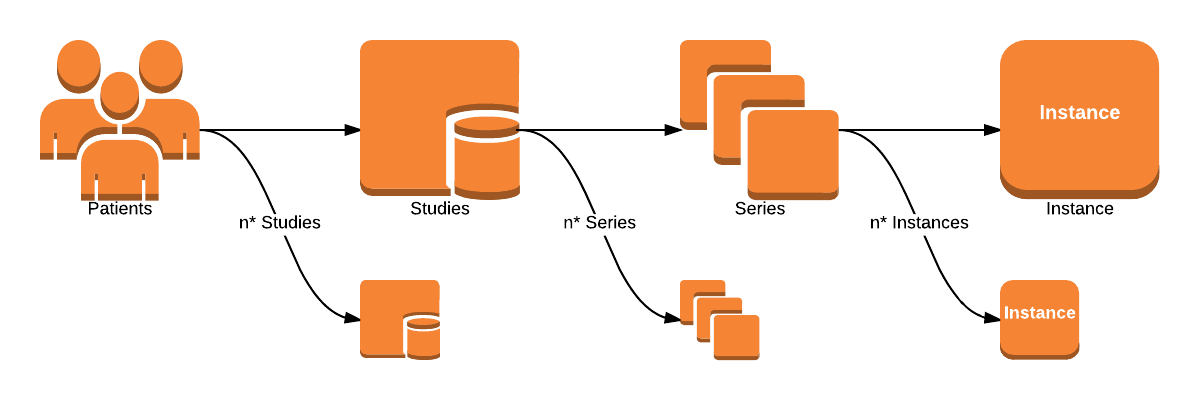
\includegraphics[width=\textwidth]{images/fig025}
\caption{[DOI: \href{https://doi.org/10.13140/RG.2.2.19014.32321}{10.13140/RG.2.2.19014.32321}] This diagram~\cite{calisto2019mips} shows that a given patient benefits from a set of medical imaging studies. Each study is made from a set of series. Each series is, in turn, a set of instances.}
\label{fig:fig025}
\end{figure}
%%%%%%%%%%%%%%%%%%%%%%%%%%%%%%%%%%%%%%%%%%%%%%%%%%%

\section{Medical Imaging Storage}
\label{sec:chap002008}

The \ac{PACS}~\cite{carter2018digital} offers efficient storage and a simple way to access the (\ac{DICOM}) images in a variety of modalities.
The deployment of these technologies requires specific packages and environments, which will be detailed below.
Our platform provides essential tools for the deployment of multimodality strategies, interactive image visualization/manipulation, and study navigation in a web browser.
This paves the road for the integration for multimodality strategies into \ac{PACS} as it only needs a web browser which is always accessible on the clinical workstations.